\documentclass[12pt]{amsart}
\usepackage{amsaddr}
\usepackage[draft]{../marktext} 
%% Remove draft for real article, put twocolumn for two columns
\usepackage[draft]{../svmacro}
\usepackage[utf8]{inputenc}
\usepackage[style=alphabetic, backend=biber]{biblatex}
\addbibresource{bibliography.bib}

%% commentary bubble
\newcommand{\SV}[2][]{\sidenote[colback=green!10]{\textbf{SV\xspace #1:} #2}}

%% Title 
\title{ Worksheet 10}
\author{MATH 101}
\address{Fulbright University, Ho Chi Minh City, Vietnam}

%\author{Co-author}
%\address{  }
%\email {  }
%
\date{\today}

\begin{document}

\maketitle

\section*{Related rates}
\begin{question}
	A 10-ft ladder is leaning against a wall. If the top of the ladder slides down the wall at a rate of 2 ft/sec, how fast is the bottom moving along the ground when the bottom of the ladder is 5 ft from the wall?
	\begin{center}
		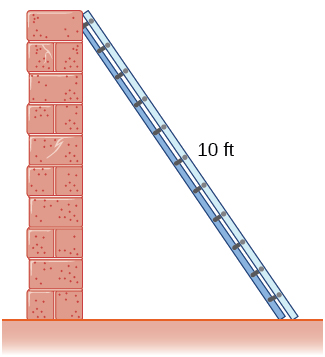
\includegraphics{fig1.jpeg}
	\end{center}
\end{question}

\newpage

\begin{question}
	A 6-ft-tall person walks away from a 10-ft lamppost at a constant rate of  3ft/sec.
	What is the rate that the tip of the shadow moves away from the pole when the person is  10ft
	away from the pole?
	\begin{center}
		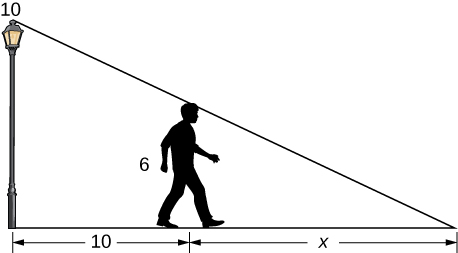
\includegraphics{fig2.jpeg}
	\end{center}
\end{question}

\newpage

\section*{Approximations}
The goal of linear approximation is to find a linear function that can best represent a function $f(x)$
near a particular point $x = a$.
It turns out, the equation for the tangent line provides the best linear approximation for $f(x)$!


If $y = f(x)$, then the linear approximation of $f(x)$ when $x = a$ is
\begin{equation*}
	L(x) = f(a) + f'(a)(x-a) \,.
\end{equation*}

\begin{question}
	\begin{enumerate}
		\item Let $f(x) = e^{x^2}$. Find $L(x)$ at $x = 1$.
		      \vspace{3cm}
		\item Invent a way to compare the error between $f(x)$ and $L(x)$ with that between $f(x)$ and $g(x) = e+ x-1$.
		      \vspace{3cm}
	\end{enumerate}


\end{question}

\newpage


The linear approximation just captures the slope of the function at a particular point.
Let's reverse engineer the problem. If you knew $L(x)$ must look something like $b(x-a) + c$, then $c$ must be $f(a)$ and and $b$ must be $f'(a)$.


If you were to use a quadratic function to approximate $f(x)$, how can you find that magical quadratic function?

\newpage






\section*{Optimization}

The meaning of second derivative is that it tells us about the concavity of the graph of a function.


\begin{center}
	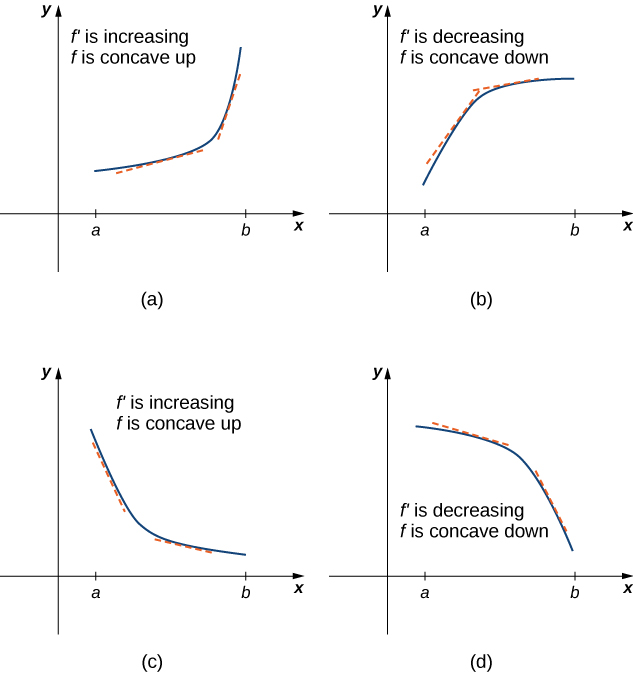
\includegraphics{fig3.jpeg}
\end{center}



\begin{definition}
	Let \( f \) be a function defined over an interval \( I \) and let \( c \in I \).
	We say \( f \) has an absolute maximum on \( I \) at \( c \) if \( f(c) \geq f(x) \) for all \( x \in I \).
	We say \( f \) has an absolute minimum on \( I \) at \( c \) if \( f(c) \leq f(x) \) for all \( x \in I \).
	If \( f \) has an absolute maximum on \( I \) at \( c \) or an absolute minimum on \( I \) at \( c \), we say \( f \) has an absolute extremum on \( I \) at \( c \).
\end{definition}


\begin{theorem}
	If \( f \) is a continuous function over the closed, bounded interval \([a, b]\),
	then there is a point in \([a, b]\) at which \( f \) has an absolute maximum over \([a, b]\),
	and there is a point in \([a, b]\) at which \( f \) has an absolute minimum over \([a, b]\).
\end{theorem}



\end{document}
